\chapter{Diseño}

Este capítulo presenta el diseño conceptual y arquitectónico de la plataforma. Se describen las decisiones fundamentales que estructuran el sistema, desde la arquitectura general y el flujo de datos hasta el diseño específico de los componentes del backend y del frontend. El propósito es establecer un marco coherente y justificado que sirva como base para la implementación técnica detallada en el capítulo siguiente.

\section{Diseño de la arquitectura}

La plataforma se fundamenta en una arquitectura cliente-servidor desacoplada, un modelo robusto y escalable que separa claramente las responsabilidades del sistema. Esta arquitectura divide la aplicación en tres componentes principales e independientes:

\begin{itemize}
    
    \item La base de datos: Contiene todos los datos médicos con lo que se va a trabajar. Es la capa de persistencia en la apliación.
    
    \item El Backend: Es el núcleo lógico de la aplicación. Se encarga de gestionar el acceso a la base de datos, procesar las consultas complejas, aplicar la lógica de negocio y exponer los datos de manera segura y estructurada a través de una API de servicio.

    \item El Frontend: Es la capa de presentación con la que interactúa el usuario. Se ejecuta en el navegador web y su única responsabilidad es solicitar los datos al backend, renderizar la interfaz de usuario y presentar las visualizaciones de datos de forma interactiva.
\end{itemize}

%\begin{figure}[H]
%    \centering
%    \fbox{\includegraphics[width=0.85\textwidth]{imagenes/frontandbackend.png}}
    %
\includegraphics[width=0.4\textwidth]{imagenes/physionet-logo.png}
%    \caption{Esquema conexiones Frontend y Backend. \cite{backfrontendfoto}.}
%\end{figure}


\begin{figure}[H]
    \centering
    \fbox{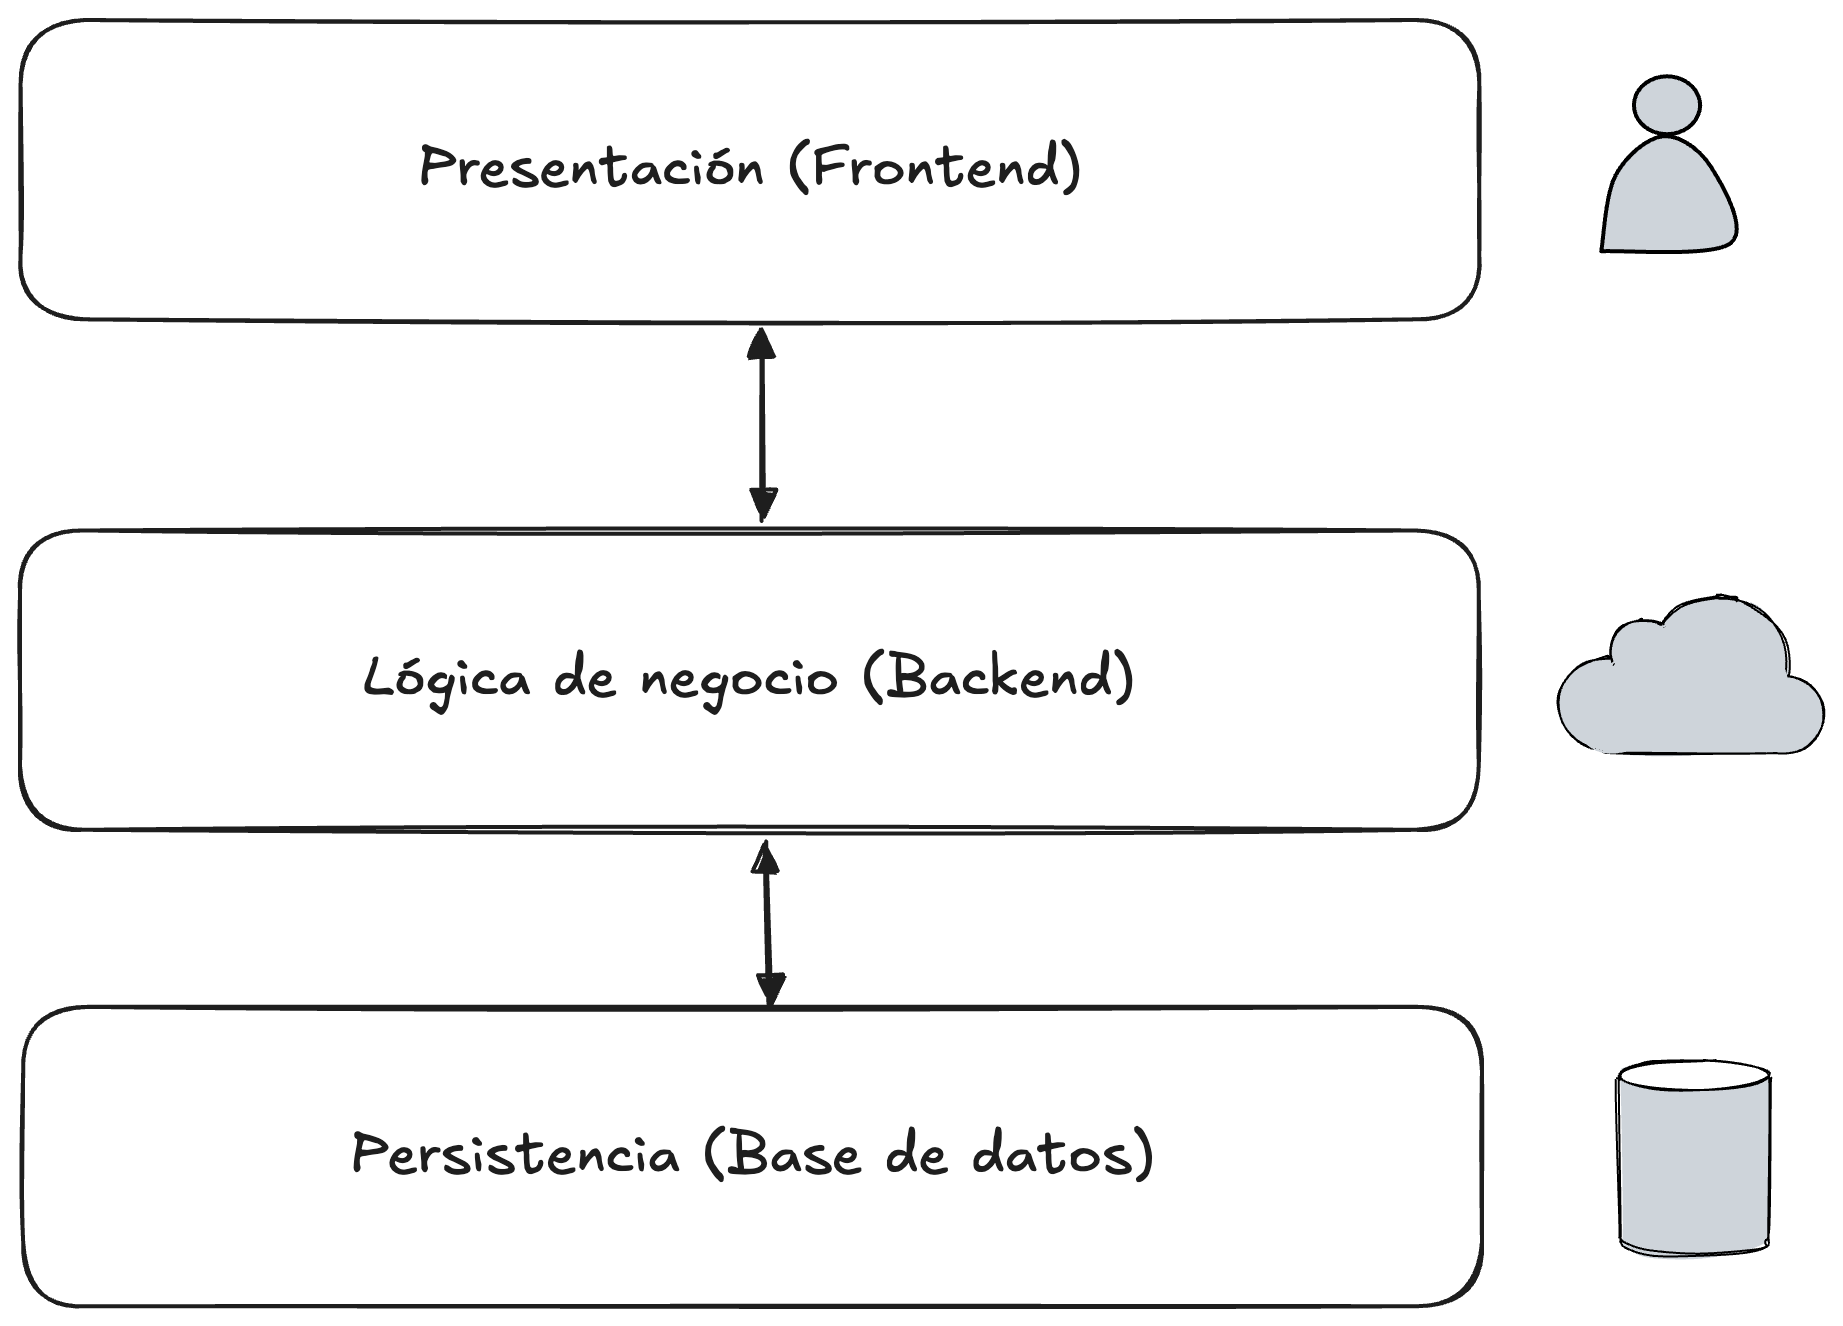
\includegraphics[width=0.85\textwidth]{imagenes/arch-dis2.png}}
    %
\includegraphics[width=0.4\textwidth]{imagenes/physionet-logo.png}
    \caption{Esquema conexiones BD, Backend y Frontend.}
\end{figure}




La elección de este modelo ofrece ventajas significativas para el proyecto. En primer lugar, la modularidad permite que el frontend y el backend se desarrollen, prueben y desplieguen de forma independiente. En segundo lugar, la escalabilidad se ve favorecida, ya que cada componente puede escalarse por separado según la demanda. Finalmente, facilita el mantenimiento y la evolución futura del sistema, ya que los cambios en una capa no impactan directamente en la otra mientras la interfaz de comunicación (la API) se mantenga estable.


El flujo de información está diseñado para ser eficiente y unidireccional. El proceso comienza cuando el usuario realiza una acción en la interfaz del frontend (por ejemplo, cargar el dashboard o buscar un paciente). Esta acción desencadena una petición HTTPS a un endpoint específico de la API del backend. El backend recibe la petición, la procesa, construye una consulta optimizada para la base de datos MongoDB, recupera los datos necesarios, los transforma al formato adecuado y los devuelve al frontend en formato JSON. Finalmente, el cliente recibe estos datos y los utiliza para actualizar la interfaz y renderizar las visualizaciones correspondientes.

%... aquí irá imagen del flujo

\section{Diseño de la Base de Datos}

A pesar de que MIMIC-IV se distribuye en un formato relacional (archivos CSV interconectados), para este proyecto se ha optado por un modelo de datos NoSQL documental. Esta decisión de diseño se justifica por varias razones clave:

\begin{itemize}
    \item Flexibilidad: Los datos clínicos son inherentemente heterogéneos. Un modelo documental permite almacenar registros con estructuras variables sin la rigidez de un esquema predefinido, facilitando la integración de diferentes tipos de datos.
    \item Rendimiento: Las consultas que requieren agregar información de múltiples fuentes (por ejemplo, obtener un paciente con todos sus ingresos, diagnósticos y pruebas) pueden resolverse de manera más eficiente en un modelo documental, evitando complejas operaciones de \textit{join} que serían necesarias en una base de datos relacional.
    \item Alineación con la aplicación: La estructura de documentos JSON de MongoDB se alinea de forma natural con los objetos de datos que se consumen en el frontend a través de la API, simplificando el intercambio de información.
\end{itemize}

\section{Diseño del Backend}

%El diseño del backend se centra en tres pilares: un modelo de datos flexible, una API de servicio bien definida y una capa de inteligencia artificial que permita la interacción en lenguaje natural.

%\subsection{Modelo de Datos}

%\subsection{Diseño de la API de Servicio}

%La comunicación entre el frontend y el backend se articula a través de una API RESTful. 
El backend es la lógica de negocio de la apliación, es la capa intermedia entre la base de datos y el frontend. Consta principalmente de una API, que actúa como un contrato bien definido, exponiendo una serie de endpoints lógicos agrupados por funcionalidad. El diseño contempla los siguientes grupos de endpoints:

\begin{itemize}
    \item Gestión de pacientes: Endpoints para obtener toda la información consolidada de un paciente específico.
    \item Estadísticas y Dashboard: Endpoints que sirven datos agregados y precalculados para ofrecer una visión general del estado de la base de datos.
    \item Visualizaciones específicas: Endpoints dedicados para cada gráfico, que devuelven los datos en el formato exacto que la visualización requiere, optimizando el rendimiento.
    \item Servicios de IA: Endpoints para interactuar con los modelos de lenguaje, como la interfaz de chat y la generación de resúmenes.
\end{itemize}

%\subsection{Diseño del Módulo de Inteligencia Artificial}
%Para integrar las capacidades de consulta en lenguaje natural, se ha diseñado un módulo que actúa como un intermediario inteligente entre un Gran Modelo de Lenguaje (LLM) y la base de datos. En lugar de permitir un acceso directo y no controlado, el diseño se basa en el paradigma de \textit{tool use} (uso de herramientas).

%Se expone un conjunto de herramientas bien definidas y seguras (p. ej., buscar documentos, contar registros, obtener esquema) que el LLM puede invocar. El diseño contempla el uso de un protocolo estandarizado como el Model Context Protocol (MCP) para gestionar esta comunicación. De este modo, cuando un usuario realiza una pregunta, el LLM no genera directamente una consulta a la base de datos, sino que decide qué herramienta utilizar y con qué parámetros, delegando la ejecución en el backend. Este enfoque garantiza un acceso seguro, controlado y auditable a los datos.

\section{Diseño del Frontend}

El diseño del frontend se enfoca en la experiencia de usuario (UX) y en la presentación clara de información clínica compleja.

%\subsection{Arquitectura de la Interfaz de Usuario (UI)}

La interfaz se construye sobre una arquitectura basada en componentes. Cada elemento de la UI, desde un simple botón hasta un gráfico complejo, es un componente autónomo, reutilizable y con una responsabilidad única. La estructura de la aplicación se organiza en vistas o páginas principales, como el \textit{Dashboard} general, la vista detallada de un \textit{Paciente} o la interfaz de \textit{Chat}.

El diseño visual sigue los principios del minimalismo, utilizando un lenguaje de diseño limpio y moderno para evitar la sobrecarga cognitiva del usuario. El objetivo es que la información y las visualizaciones sean las protagonistas, facilitando la interpretación de los datos sin distracciones innecesarias.

%\subsection{Estrategia de Visualización de Datos}

%Se ha diseñado una estrategia de visualización dual para equilibrar la velocidad de desarrollo con la capacidad de personalización.
%\begin{itemize}
%    \item Para gráficos estándar (p. ej., diagramas de barras, pirámides poblacionales), se opta por librerías declarativas de alto nivel como Observable Plot. Estas herramientas permiten generar visualizaciones comunes con un código conciso y mantenible.
%    \item Para visualizaciones complejas y personalizadas (p. ej., diagramas de cuerdas, sunbursts interactivos), que requieren un control granular sobre cada elemento gráfico, se recurre a librerías de bajo nivel como D3.js.
%\end{itemize}
%Este enfoque híbrido permite desarrollar rápidamente las visualizaciones más comunes, reservando el esfuerzo para aquellas que aportan un valor analítico único y requieren una implementación a medida.

